\let\negmedspace\undefined
\let\negthickspace\undefined
\documentclass[journal]{IEEEtran}
\usepackage[a5paper, margin=10mm, onecolumn]{geometry}
%\usepackage{lmodern} % Ensure lmodern is loaded for pdflatex
\usepackage{tfrupee} % Include tfrupee package

\setlength{\headheight}{1cm} % Set the height of the header box
\setlength{\headsep}{0mm}     % Set the distance between the header box and the top of the text

\usepackage{gvv-book}
\usepackage{gvv}
\usepackage{cite}
\usepackage{amsmath,amssymb,amsfonts,amsthm}
\usepackage{algorithmic}
\usepackage{graphicx}
\usepackage{textcomp}
\usepackage{xcolor}
\usepackage{txfonts}
\usepackage{listings}
\usepackage{enumitem}
\usepackage{mathtools}
\usepackage{gensymb}
\usepackage{comment}
\usepackage[breaklinks=true]{hyperref}
\usepackage{tkz-euclide} 
\usepackage{listings}
% \usepackage{gvv}                                        
\def\inputGnumericTable{}                                 
\usepackage[latin1]{inputenc}                                
\usepackage{color}                                            
\usepackage{array}                                            
\usepackage{longtable}                                       
\usepackage{calc}                                             
\usepackage{multirow}                                         
\usepackage{hhline}                                           
\usepackage{ifthen}                                           
\usepackage{lscape}
\begin{document}

\bibliographystyle{IEEEtran}
\vspace{3cm}

\title{1-1.2-20}
\author{EE24BTECH11064 - Harshil Rathan 
}
% \maketitle
% \newpage
% \bigskip
{\let\newpage\relax\maketitle}

\renewcommand{\thefigure}{\theenumi}
\renewcommand{\thetable}{\theenumi}
\setlength{\intextsep}{10pt} % Space between text and floats


\numberwithin{equation}{enumi}
\numberwithin{figure}{enumi}
\renewcommand{\thetable}{\theenumi}
\textbf{Question}:\\
Three vertices of a prallelogram $ABCD$ are \textbf{A} \brak{3,-1,2},\textbf{B} \brak{1,-2,4} and \textbf{C} \brak{-1,1,2}.Find the coordinates of the fourth vertex.
\\
\textbf{Solution: }
\begin{table}[h!]    
  \centering
  \begin{tabular}[12pt]{ |c| c|}
    \hline
    \textbf{Equations}& \textbf{Given}\\ 
    \hline
     $2y$ & $3x+12$ \\
    \hline 
     $x$ & $2, 8 $\\
    \hline
    \end{tabular}
    \caption{Given Equations}

\end{table}
\begin{align}
    \vec{M} = \frac{\vec{A}+\vec{C}}{2}\\
    \vec{P} = \frac{\vec{B}+\vec{D}}{2}\\
    \vec{M} = \vec{P}
\end{align}    
\begin{align}    
\myvec{M}=\frac{\myvec{3\\-1\\2}+\myvec{-1\\1\\2}}{2}\\\\
M =\myvec{1\\0\\2}\\
\end{align}
\begin{align}
\myvec{P}=\frac{\myvec{1\\-2\\4}+\myvec{x\\y\\z}}{2}\\\\
P= \myvec{\frac{1+x}{2}\\ \frac{y-2}{2} \\ \frac{z+4}{2}}\\
\end{align}
\begin{align}
\vec{M} = \vec{P} \\
\end{align}
On comparing both sides, 
\begin{align}
x=1, y=2, z=0
\end{align}
\begin{figure}[h!]
   \centering
   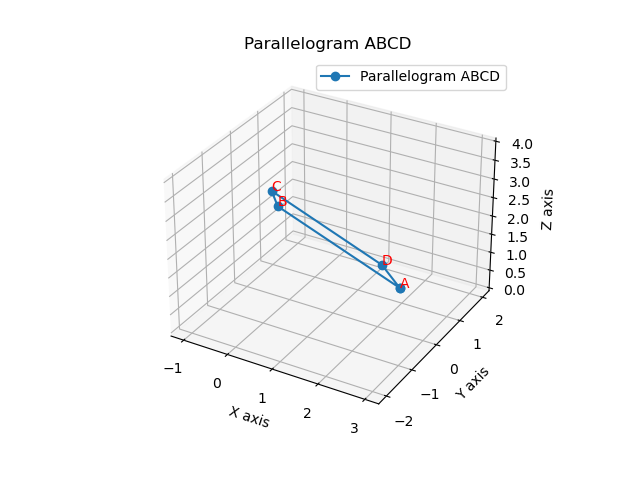
\includegraphics[width=0.7\linewidth]{figs/Figure_1.png}
   \caption{Stem Plot of y\brak{n}}
   \label{stemplot}
\end{figure}





\end{document}
